\documentclass[a4paper]{article}
%\usepackage{enumitem, amsmath, gensymb, graphicx, caption, amssymb, geometry, fancyhdr, arydshln, adjustbox,float}
\usepackage{enumitem, amsmath, geometry, fancyhdr, amssymb, float, adjustbox}

\geometry{left=1in, right=1in, top=1in, bottom=1in}
\pagestyle{fancy}

\newcommand{\myName}{\textbf{Shantanu Ghodgaonkar}\\\textit{Univ ID}: N11344563\\\textit{Net ID}: sng8399\\\textit{Ph.No.}: +1 (929) 922-0614}
\newlist{qalist}{description}{1}
\setlist[qalist]{style=unboxed,leftmargin=0.5cm,labelwidth=2.5cm}


\title{Homework 5 Answers : ROB-GY 6103}
\author{\myName}
\date{\today}

\fancyhead{} % Clear existing header settings 
\fancyhead[L]{\today}
\fancyhead[R]{N11344563}


\begin{document}
	
	\begin{titlepage}
	    \centering
	    \vspace{2cm}
	    \Huge\textbf{Mathematics for Robotics \\ ROB-GY 6103 \\ Homework 5 Answers}
	    \vspace{1cm}
	    \\ \Large \today
	    \vfill
	    \Large \myName
	\end{titlepage}
	
	\begin{qalist}			
		\item[Question: 2.] \setcounter{equation}{0}
		\item[Answer:] We are given the matrix, 
			\begin{equation}
				A = \begin{bmatrix}1 & 0 & \sqrt{2} \\ 0 & 2 & 0 \\ \sqrt{2} & 0 & 0\end{bmatrix}
			\end{equation}
			
			It gives us the three eigenvalues, 
			 \begin{align}
				 {\lambda}_{1} &= 2 \notag \\ {\lambda}_{2} &= 2 \\ {\lambda}_{3} &= -1 \notag \\ \Rightarrow \Lambda &= \begin{bmatrix} 2 & 0 & 0\\ 0 & 2 & 0 \\ 0 & 0 & -1 \end{bmatrix}
			\end{align} 
			
			Using MATLAB, we can find the three eigenvectors to be, 
			\begin{align}
				{v}^{1} &= \begin{bmatrix}  0.57 \\ 0 \\ -0.81 \end{bmatrix} ,~{v}^{2} = \begin{bmatrix}  0.81 \\ 0 \\ 0.57 \end{bmatrix}  ,~{v}^{3} = \begin{bmatrix}  0 \\ 1 \\ 0 \end{bmatrix}\\ 
				V &=  \begin{bmatrix} 0.57 & 0.81 & 0 \\ 0 & 0 & 1 \\ -0.81 & 0.57 & 0 \end{bmatrix}
			\end{align}
			
			We can see that, 
			\begin{equation}
				{V}^{-1} = \begin{bmatrix}0.57 & 0 & -0.81 \\ 0.81 & 0 & 0.57 \\ 0 & 1 & 0 \end{bmatrix} = {V}^{T} \Rightarrow \textit{$V$ is Orthogonal}
			\end{equation}
			
			By multiplying the matrices $V \Lambda {V}^{T} \rightarrow$ 
			\begin{align}
				V \Lambda {V}^{T} &=  \begin{bmatrix} 0.57 & 0.81 & 0 \\ 0 & 0 & 1 \\ -0.81 & 0.57 & 0 \end{bmatrix}   \begin{bmatrix} 2 & 0 & 0\\ 0 & 2 & 0 \\ 0 & 0 & -1 \end{bmatrix}    \begin{bmatrix}0.57 & 0 & -0.81 \\ 0.81 & 0 & 0.57 \\ 0 & 1 & 0 \end{bmatrix} \\ 
				&=  \begin{bmatrix}1 & 0 & \sqrt{2} \\ 0 & 2 & 0 \\ \sqrt{2} & 0 & 0\end{bmatrix} \\ 
				&= A
			\end{align}
			$\therefore$ we can see that the statement \emph{even with repeated e-values, we can still diagonalize a symmetric matrix using orthogonal matrices} is true using above numerical example.
			
			
		\item[Question: 4.a.] \setcounter{equation}{0}
		\item[Answer:] n = 99
		
		\newpage
		
		\item[Question: 4.b.] \setcounter{equation}{0}
		\item[Answer:] Given below is the plot of the Norm error in x-hat using Batch Process -
			\begin{figure}[H]			
				\vspace{0.5cm}
				\centering
				\fbox{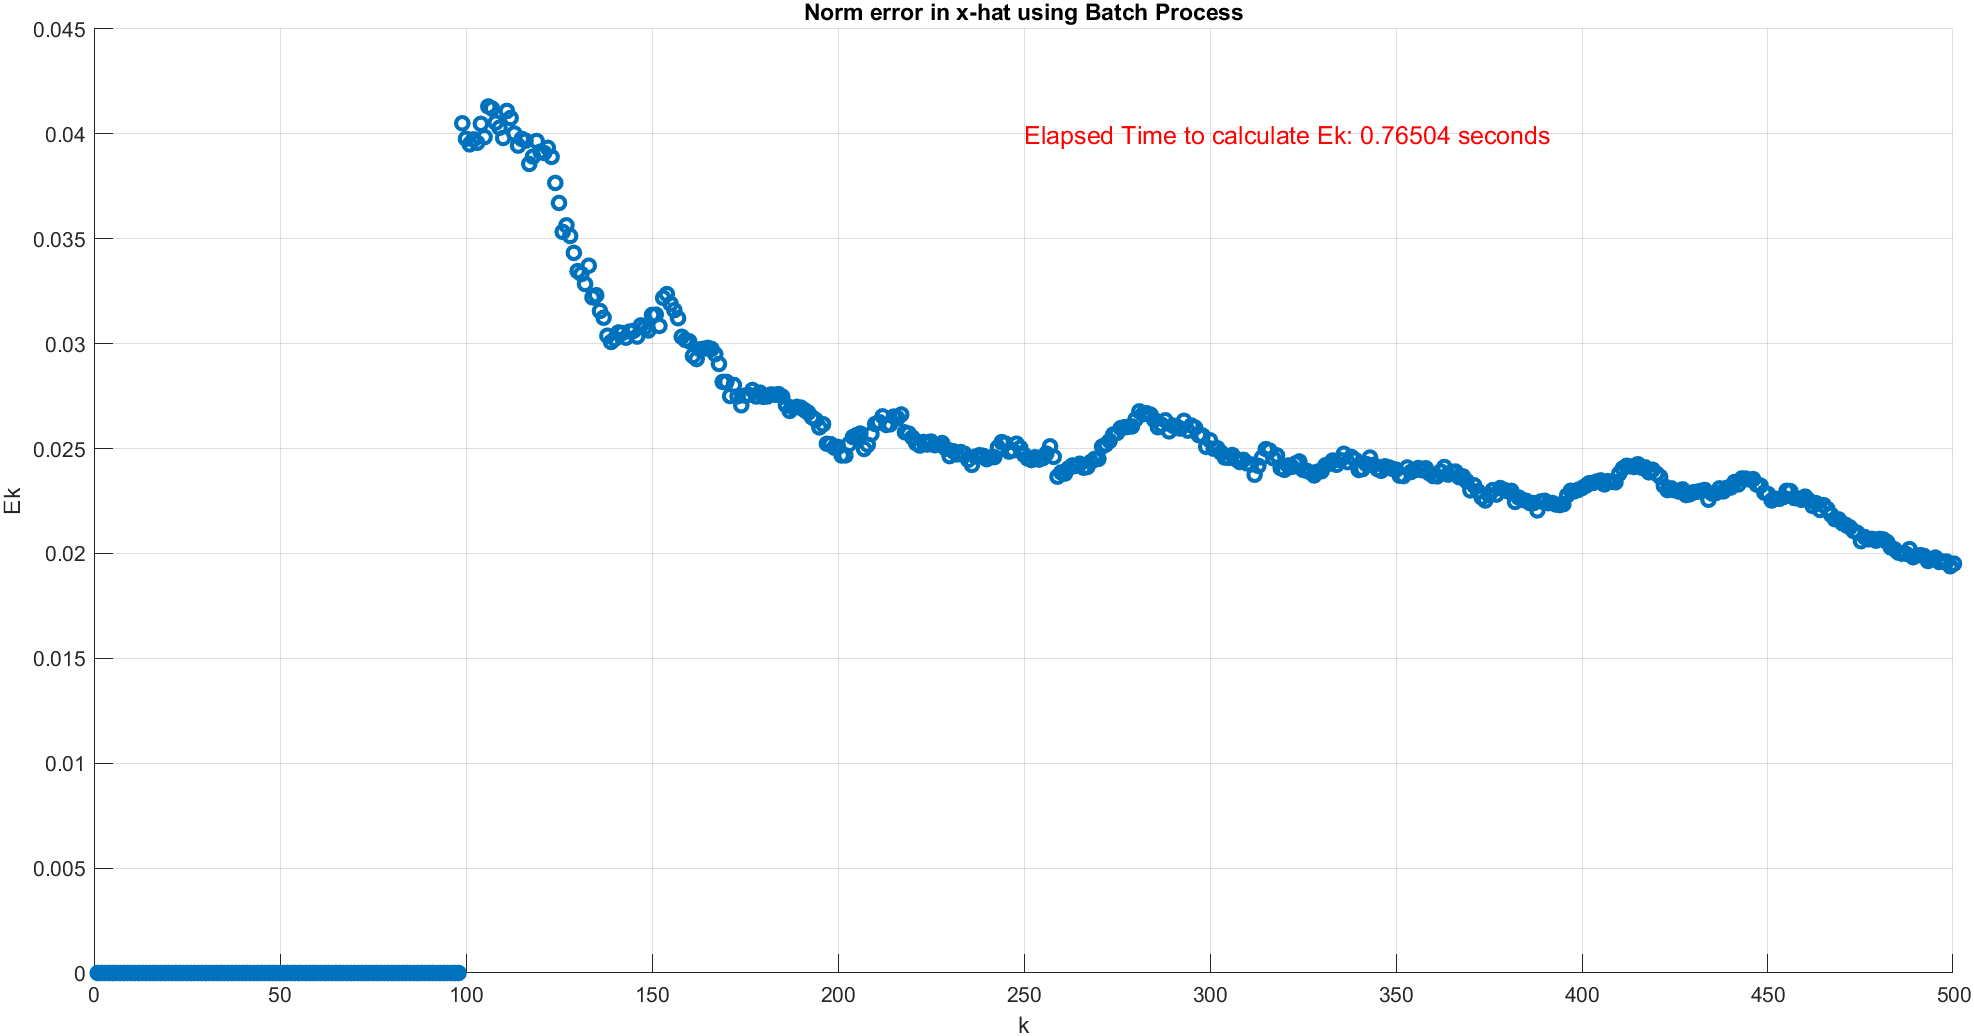
\includegraphics[width=0.75\textwidth]{q4b.png}}
				\caption{Norm error in x-hat using Batch Process} 
				\label{fig:q4b}
				\vspace{0.5cm}
			\end{figure}
		
		\item[Question: 4.c.] \setcounter{equation}{0}
		\item[Answer:] Given below is the plot of the Norm error in x-hat using Reecursive Least Squares without Matrix Inversion Lemma
			\begin{figure}[H]			
				\vspace{0.5cm}
				\centering
				\fbox{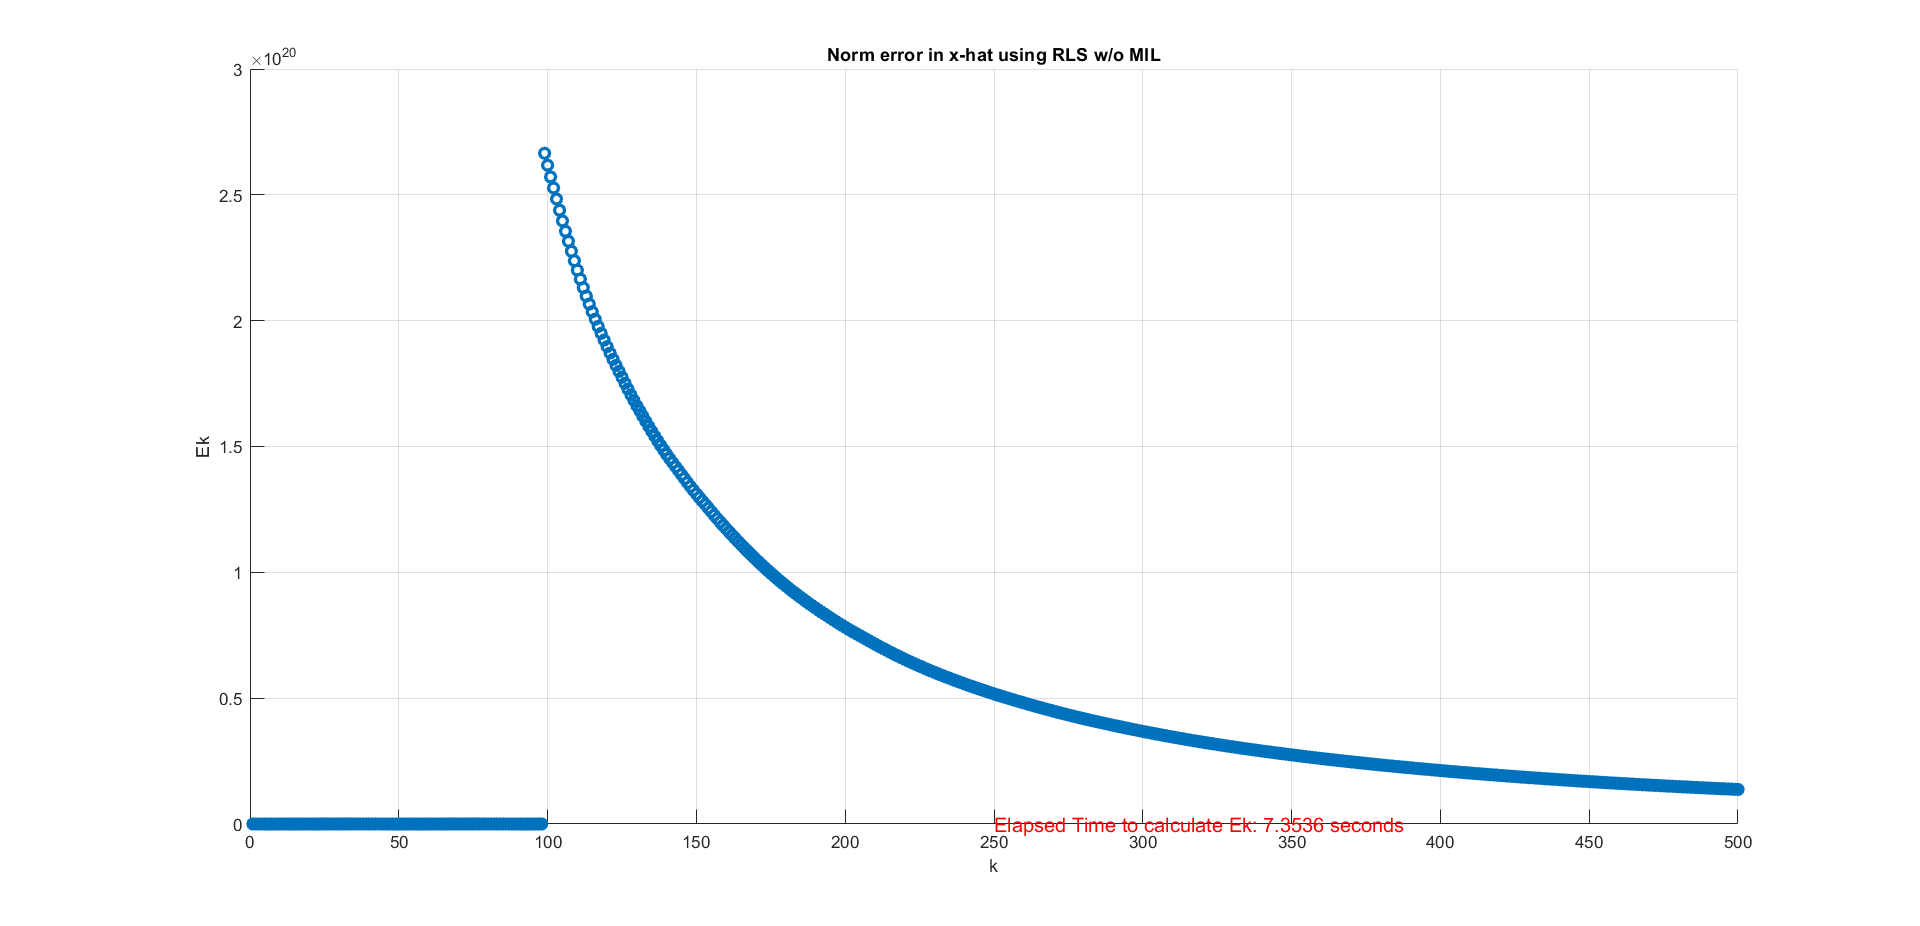
\includegraphics[width=0.75\textwidth]{q4c.png}}
				\caption{Norm error in x-hat using RLS w/o MIL} 
				\label{fig:q4b}
				\vspace{0.5cm}
			\end{figure}
		
		\newpage
		
		\item[Question: 4.d.] \setcounter{equation}{0}
		\item[Answer:] Given below is the plot of the Norm error in x-hat using Recursive Least Squares with using Matrix Inversion Lemma
			\begin{figure}[H]			
				\vspace{0.5cm}
				\centering
				\fbox{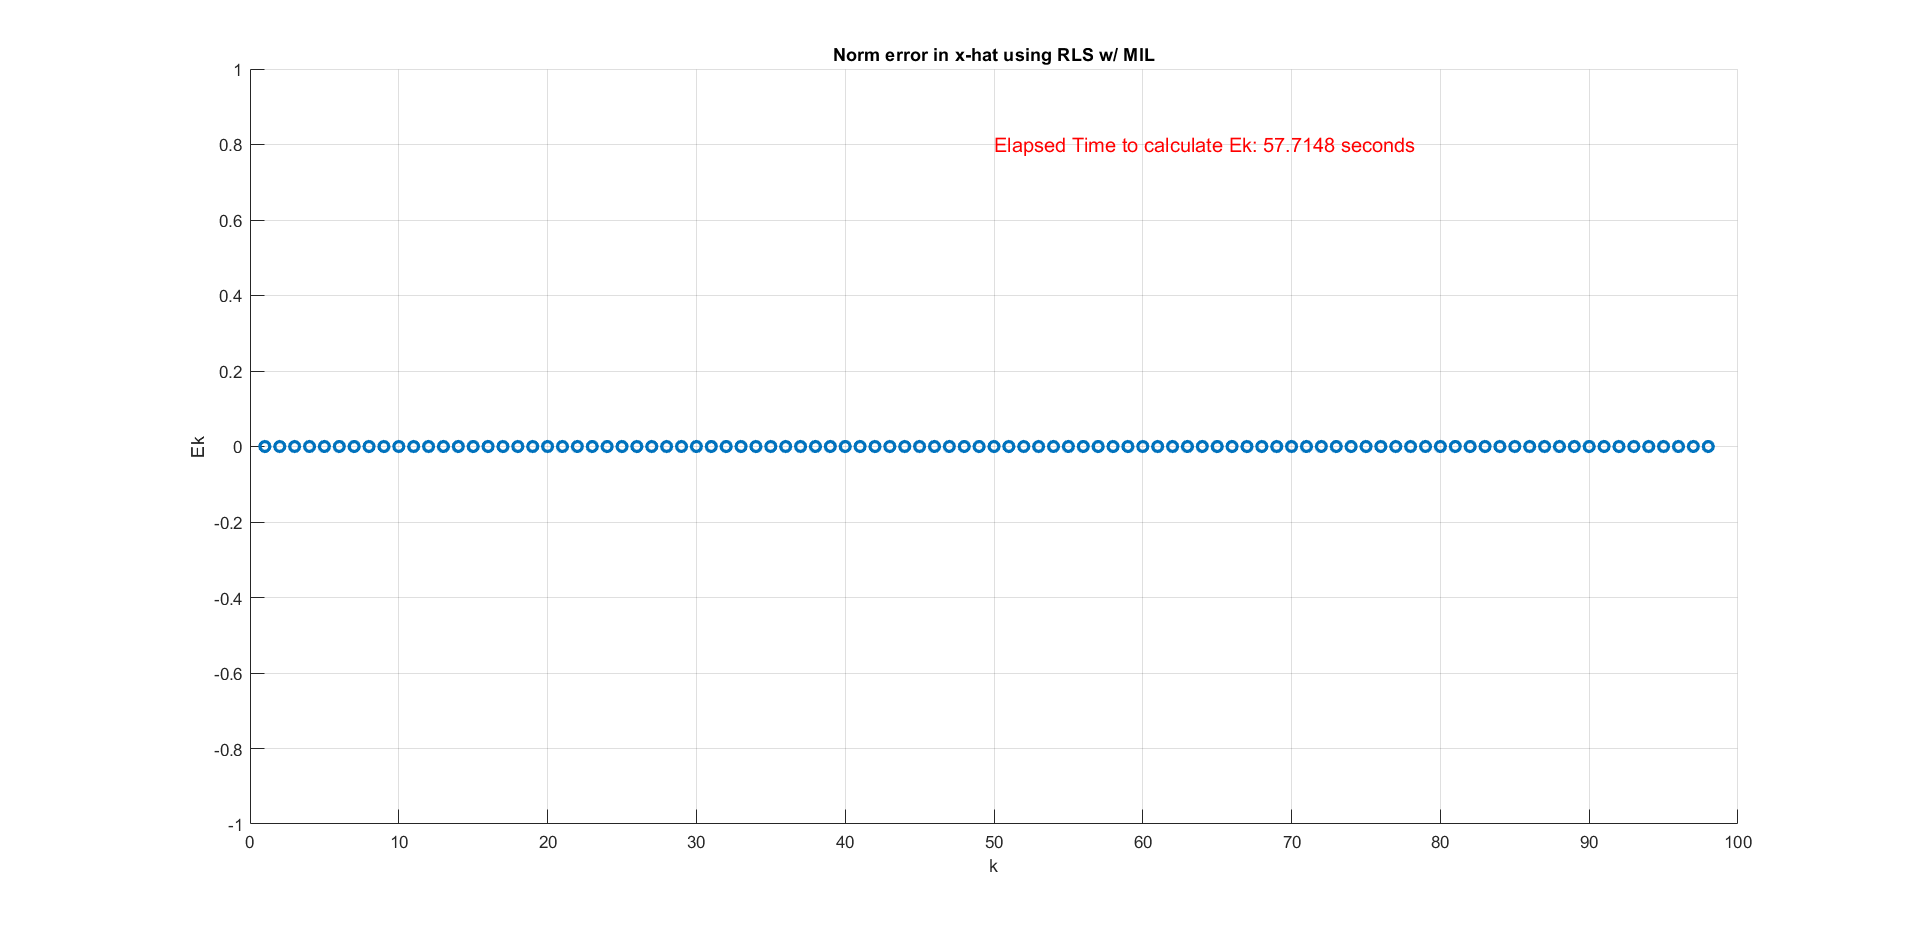
\includegraphics[width=0.75\textwidth]{q4d.png}}
				\caption{Norm error in x-hat using Recursive Least Squares with using Matrix Inversion Lemma} 
				\label{fig:q4d}
				\vspace{0.5cm}
			\end{figure}
			
		\item[Question: 5.a.] \setcounter{equation}{0}
		\item[Answer:] n = 18
		
		\item[Question: 5.b.] \setcounter{equation}{0}
		\item[Answer:] Given below is the plot of the Norm error in x-hat using Batch Process -
			\begin{figure}[H]			
				\vspace{0.5cm}
				\centering
				\fbox{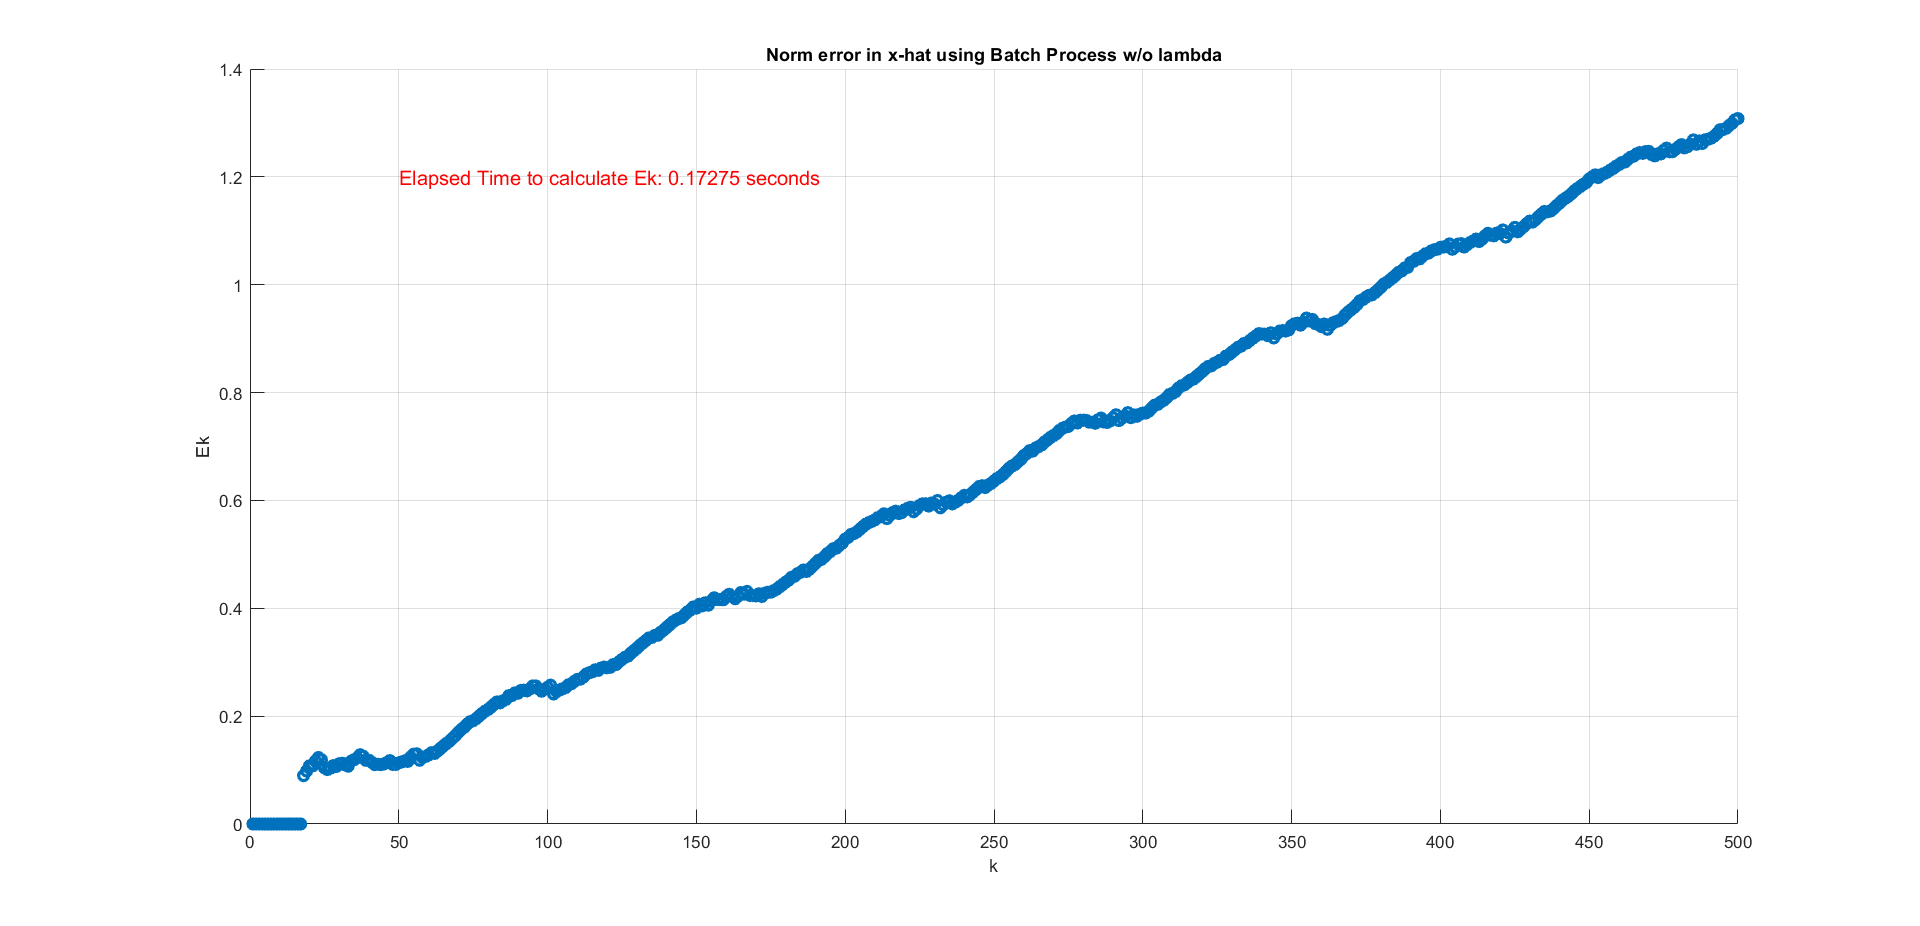
\includegraphics[width=0.75\textwidth]{q5b.png}}
				\caption{Norm error in x-hat using Batch Process} 
				\label{fig:q5b}
				\vspace{0.5cm}
			\end{figure}

		\newpage

		\item[Question: 5.c.] \setcounter{equation}{0}
		\item[Answer:] Given below is the plot of the Norm error in x-hat using Batch Process but using Forgetting Factor
			\begin{figure}[H]			
				\vspace{0.5cm}
				\centering
				\fbox{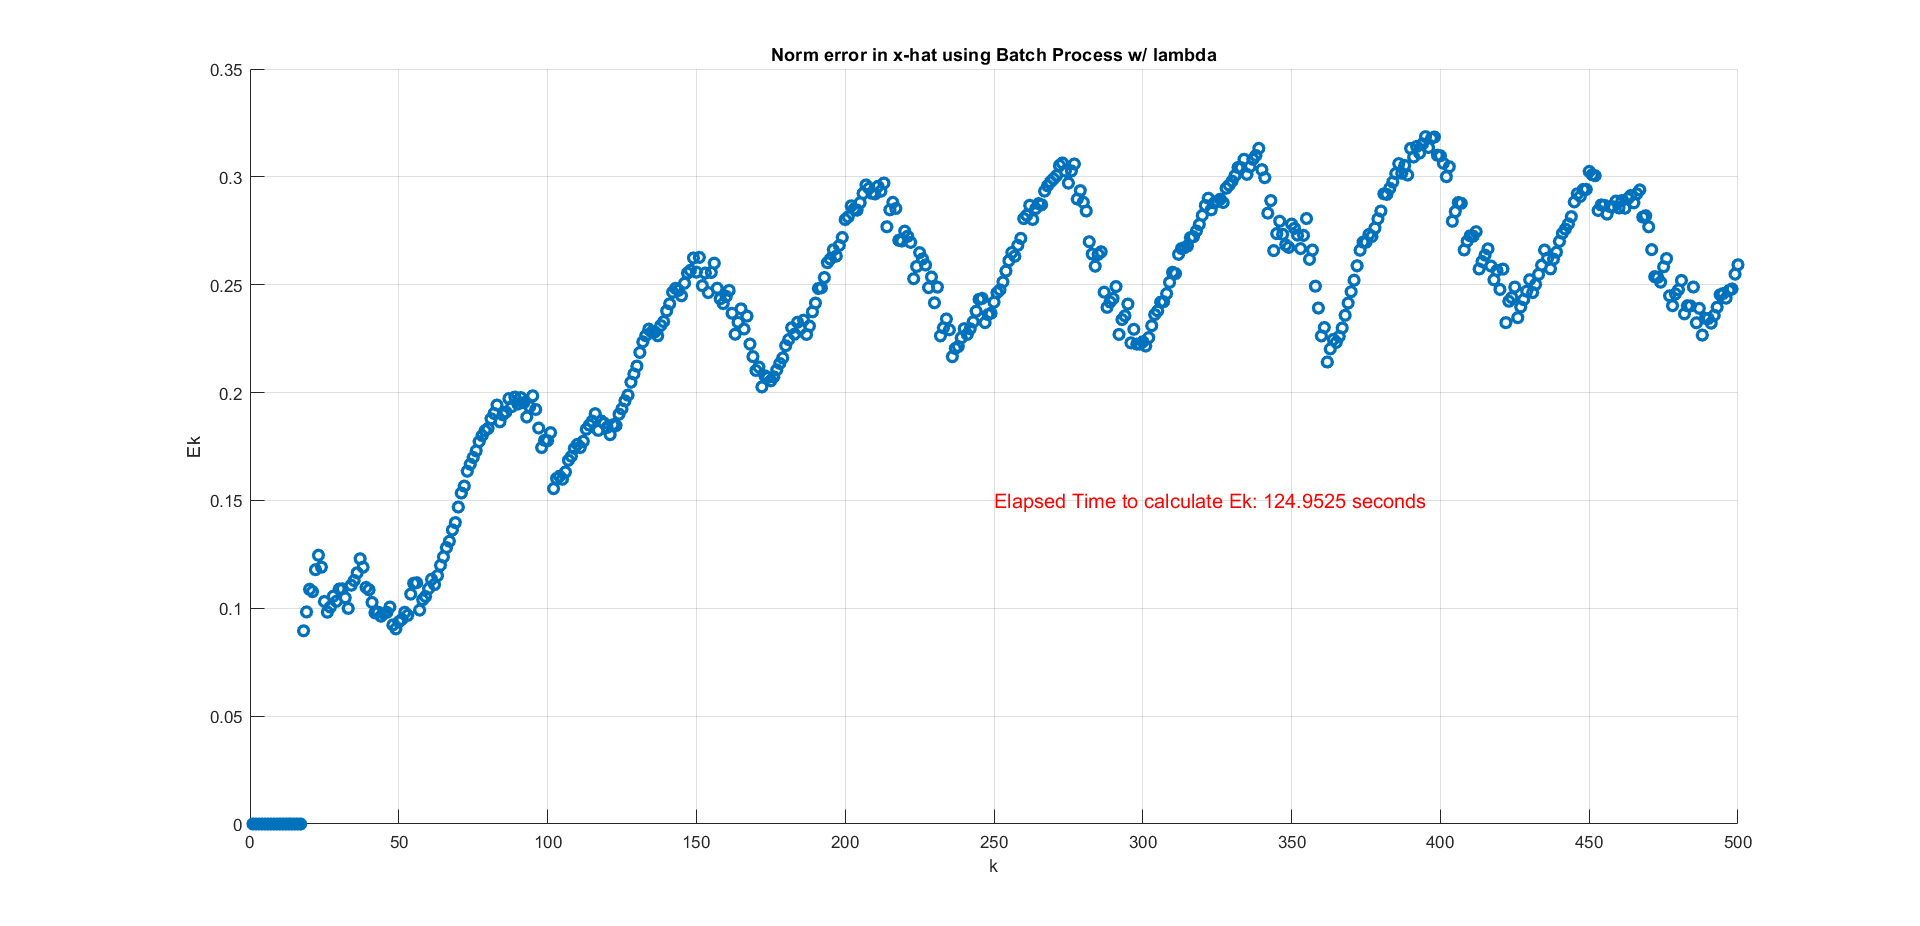
\includegraphics[width=0.75\textwidth]{q5c.png}}
				\caption{Norm error in x-hat using Batch Process and Forgetting Factor} 
				\label{fig:q5b}
				\vspace{0.5cm}
			\end{figure}
		
		\item[Question: 5.d.] \setcounter{equation}{0}
		\item[Answer:] Given below is the plot of the Norm error in x-hat using Reecursive Least Squares with using Matrix Inversion Lemma but using Forgetting Factor
			\begin{figure}[H]			
				\vspace{0.5cm}
				\centering
				\fbox{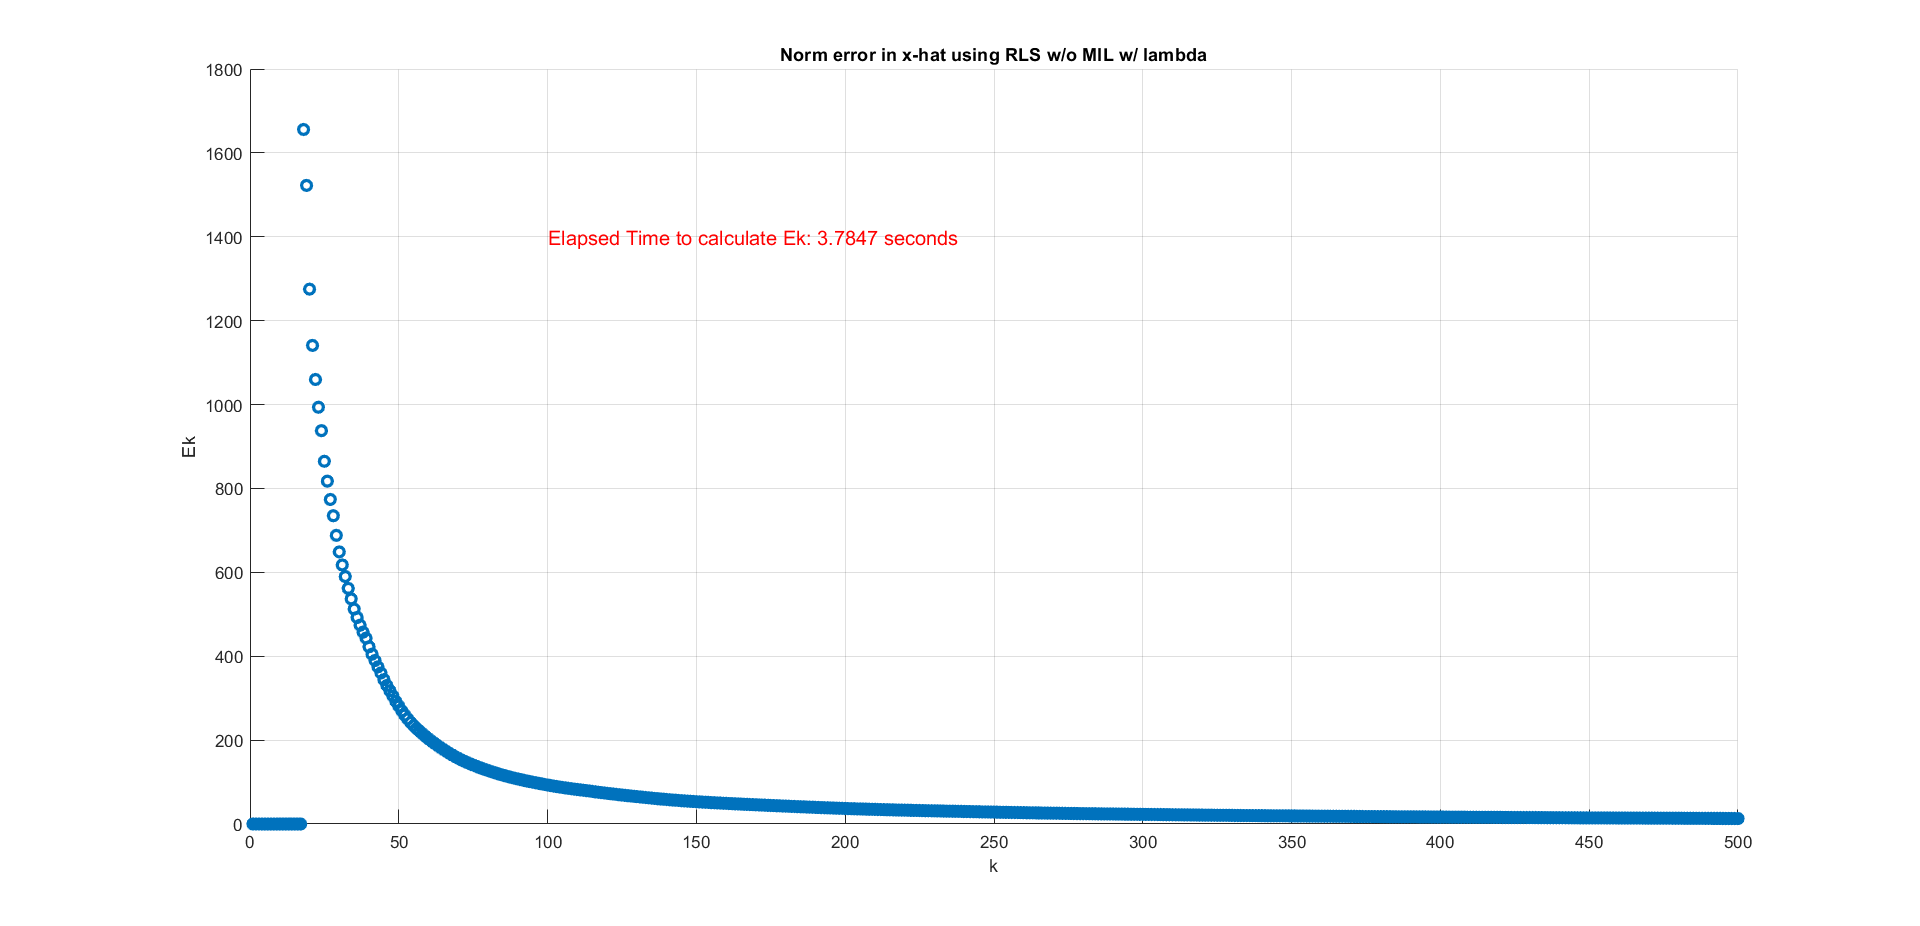
\includegraphics[width=0.75\textwidth]{q5d.png}}
				\caption{Norm error in x-hat using Reecursive Least Squares with using Matrix Inversion Lemma but using Forgetting Factor} 
				\label{fig:q5d}
				\vspace{0.5cm}
			\end{figure}
	\end{qalist}
\end{document}